%-----------------------------------------------------------------------------%


\chapter{\babDua}
%-----------------------------------------------------------------------------%
Bab ini membahas analisis kebutuhan sistem, alur kerja sistem lama vs sistem baru, serta perancangan teknis arsitektur website menggunakan framework Django.

\section{Dasar Teknologi yang Digunakan}
Pengembangan sistem informasi website laboratorium ini dibangun di atas serangkaian teknologi modern yang terintegrasi untuk memastikan keandalan, skalabilitas, dan kemudahan pemeliharaan. Bagian ini menguraikan teknologi utama yang digunakan baik pada sisi \textit{backend} maupun \textit{frontend}, serta mekanisme otomatisasi yang diterapkan.

\subsection{Framework Django}
Sisi \textit{backend} atau sisi server dari aplikasi ini dikembangkan menggunakan \textbf{Django}, sebuah kerangka kerja (\textit{framework}) web tingkat tinggi yang berbasis bahasa pemrograman Python. Pemilihan Django didasarkan pada arsitektur \textit{Model-View-Template} (MVT) yang mempromosikan pengembangan cepat dan desain yang bersih \cite{django2024}. Beberapa fitur kunci Django yang dimanfaatkan dalam sistem ini meliputi:
\begin{itemize}
    \item \textbf{Django ORM (\textit{Object-Relational Mapper}):} Memungkinkan interaksi dengan basis data (PostgreSQL) menggunakan objek Python tanpa perlu menulis kueri SQL secara manual. Hal ini diterapkan pada model data seperti \textit{FacultyMembers}, \textit{CurrentStudents}, dan \textit{Event}.
    \item \textbf{Django Admin Interface:} Menyediakan antarmuka manajemen konten siap pakai yang memungkinkan administrator untuk mengelola data dosen, mahasiswa, dan acara tanpa memerlukan keahlian teknis pemrograman.
    \item \textbf{Keamanan:} Django memiliki perlindungan bawaan terhadap berbagai kerentanan keamanan web umum, seperti \textit{SQL Injection}, \textit{Cross-Site Scripting} (XSS), dan \textit{Cross-Site Request Forgery} (CSRF).
\end{itemize}

\subsection{HTML, CSS, dan JavaScript}
Antarmuka pengguna (\textit{frontend}) dibangun menggunakan teknologi standar web untuk memastikan kompatibilitas lintas peramban (\textit{browser}):
\begin{itemize}
    \item \textbf{HTML (\textit{HyperText Markup Language}):} Digunakan sebagai kerangka struktur semantik halaman web, dikelola melalui sistem \textit{templating} Django.
    \item \textbf{CSS (\textit{Cascading Style Sheets}):} Digunakan untuk mengatur tata letak, warna, dan tipografi agar tampilan website responsif dan estetis pada berbagai ukuran layar, baik desktop maupun perangkat seluler.
    \item \textbf{JavaScript:} Digunakan untuk memberikan interaktivitas pada sisi klien, seperti validasi formulir dinamis dan manipulasi elemen DOM (\textit{Document Object Model}) tanpa perlu memuat ulang halaman secara keseluruhan.
\end{itemize}

\subsection{APScheduler untuk Penjadwalan Tugas}
Untuk menangani tugas-tugas latar belakang (\textit{background tasks}) yang perlu berjalan secara otomatis dan berkala, sistem ini menggunakan pustaka \textbf{APScheduler} (\textit{Advanced Python Scheduler}) \cite{apscheduler}. 
Dalam konteks aplikasi ini, APScheduler berfungsi sebagai pengganti \textit{Cron job} sistem operasi yang terintegrasi langsung dengan aplikasi Python. Fungsi utamanya adalah memicu skrip otomatisasi pada interval waktu tertentu (misalnya, setiap minggu atau setiap hari) untuk memperbarui data publikasi dan menyinkronkan data eksternal, memastikan informasi di website selalu mutakhir tanpa intervensi manual administrator.

\subsection{Integrasi Google Sheets}
Sistem ini mengimplementasikan integrasi dengan \textbf{Google Sheets API} untuk memudahkan proses input data massal. Mengingat format data akademik sering kali dikelola dalam bentuk \textit{spreadsheet}, fitur ini memungkinkan administrator atau staf pengajar untuk memperbarui data (seperti daftar mahasiswa atau jadwal seminar) melalui Google Sheets yang sudah familiar. 
Sistem kemudian secara otomatis membaca (men-\textit{fetch}) data dari \textit{sheet} tersebut dan menyimpannya ke dalam basis data aplikasi, menjembatani kemudahan penggunaan \textit{spreadsheet} dengan struktur basis data relasional.

\subsection{\textit{Publication Scraping} Menggunakan OpenAlex}
Untuk menampilkan portofolio penelitian laboratorium secara otomatis, sistem ini memanfaatkan API dari \textbf{OpenAlex}. OpenAlex adalah katalog indeksasi karya ilmiah global yang bersifat terbuka (\textit{open source}).
Mekanisme kerjanya adalah sebagai berikut:
\begin{enumerate}
    \item Sistem mengirimkan permintaan ke API OpenAlex berdasarkan nama atau ID penulis (\textit{Author ID}) dari anggota fakultas.
    \item OpenAlex mengembalikan metadata publikasi, termasuk judul, tahun terbit, nama jurnal, jumlah sitasi, dan DOI.
    \item Data tersebut diproses dan disimpan ke dalam model \texttt{PublicationOpenAlex} di database lokal.
\end{enumerate}
Pendekatan ini jauh lebih efisien dan akurat dibandingkan teknik \textit{web scraping} tradisional yang berbasis HTML, serta memastikan kepatuhan terhadap standar penggunaan data publik.

\section{Analisis Sistem}
\subsection{Analisis Sistem Berjalan}
Bagian ini membedah alur kerja pada website lama (PHP Statis) untuk memperjelas inefisiensi yang terjadi.

Proses saat ini adlaah untuk menambahkan konten pada website harus mengedit folder website secara langsung. 
Kelemahan Sistem :
\begin{enumerate}
    \item Waktu update konten lambat
    \item Risiko syntax error saat edit langsung.
    \item tidak ada manajemen pengguna
\end{enumerate}

\subsection{Analisis Kebutuhan Sistem Baru}
\begin{enumerate}[label=\Alph*.]
\item Sisi Pengunjung (Front-End):
\begin{itemize}
        \item Dapat melihat daftar berita atau acara dari lab IR-NLP terkini.
        \item Dapat melihat topik yang terkait dengan lab IR-NLP.
        \item Dapat melihat publikasi terbaru dari lab IR-NLP.
        \item Tampilan responsif (ponsel/desktop).
\end{itemize}
\item Sisi Administrator (Back-End / Django Admin):
        \begin{itemize}
            \item Login aman (autentikasi).
            \item Manajemen konten (CRUD).
            \item Manajemen kategori acara.
            \item Upload gambar/media.
            \item Upload Publikasi 
            \item Otomasi Publikasi
            \item Manajemen user admin.
        \end{itemize}
\end{enumerate}

\section{Perancangan Basis Data}
Karena menggunakan Django, perancangan ini akan direpresentasikan dalam bentuk Model.
\subsection{Entity Relationship Diagram (ERD)}
Menggambarkan hubungan antar data.

\begin{figure}[H]
    \centering
    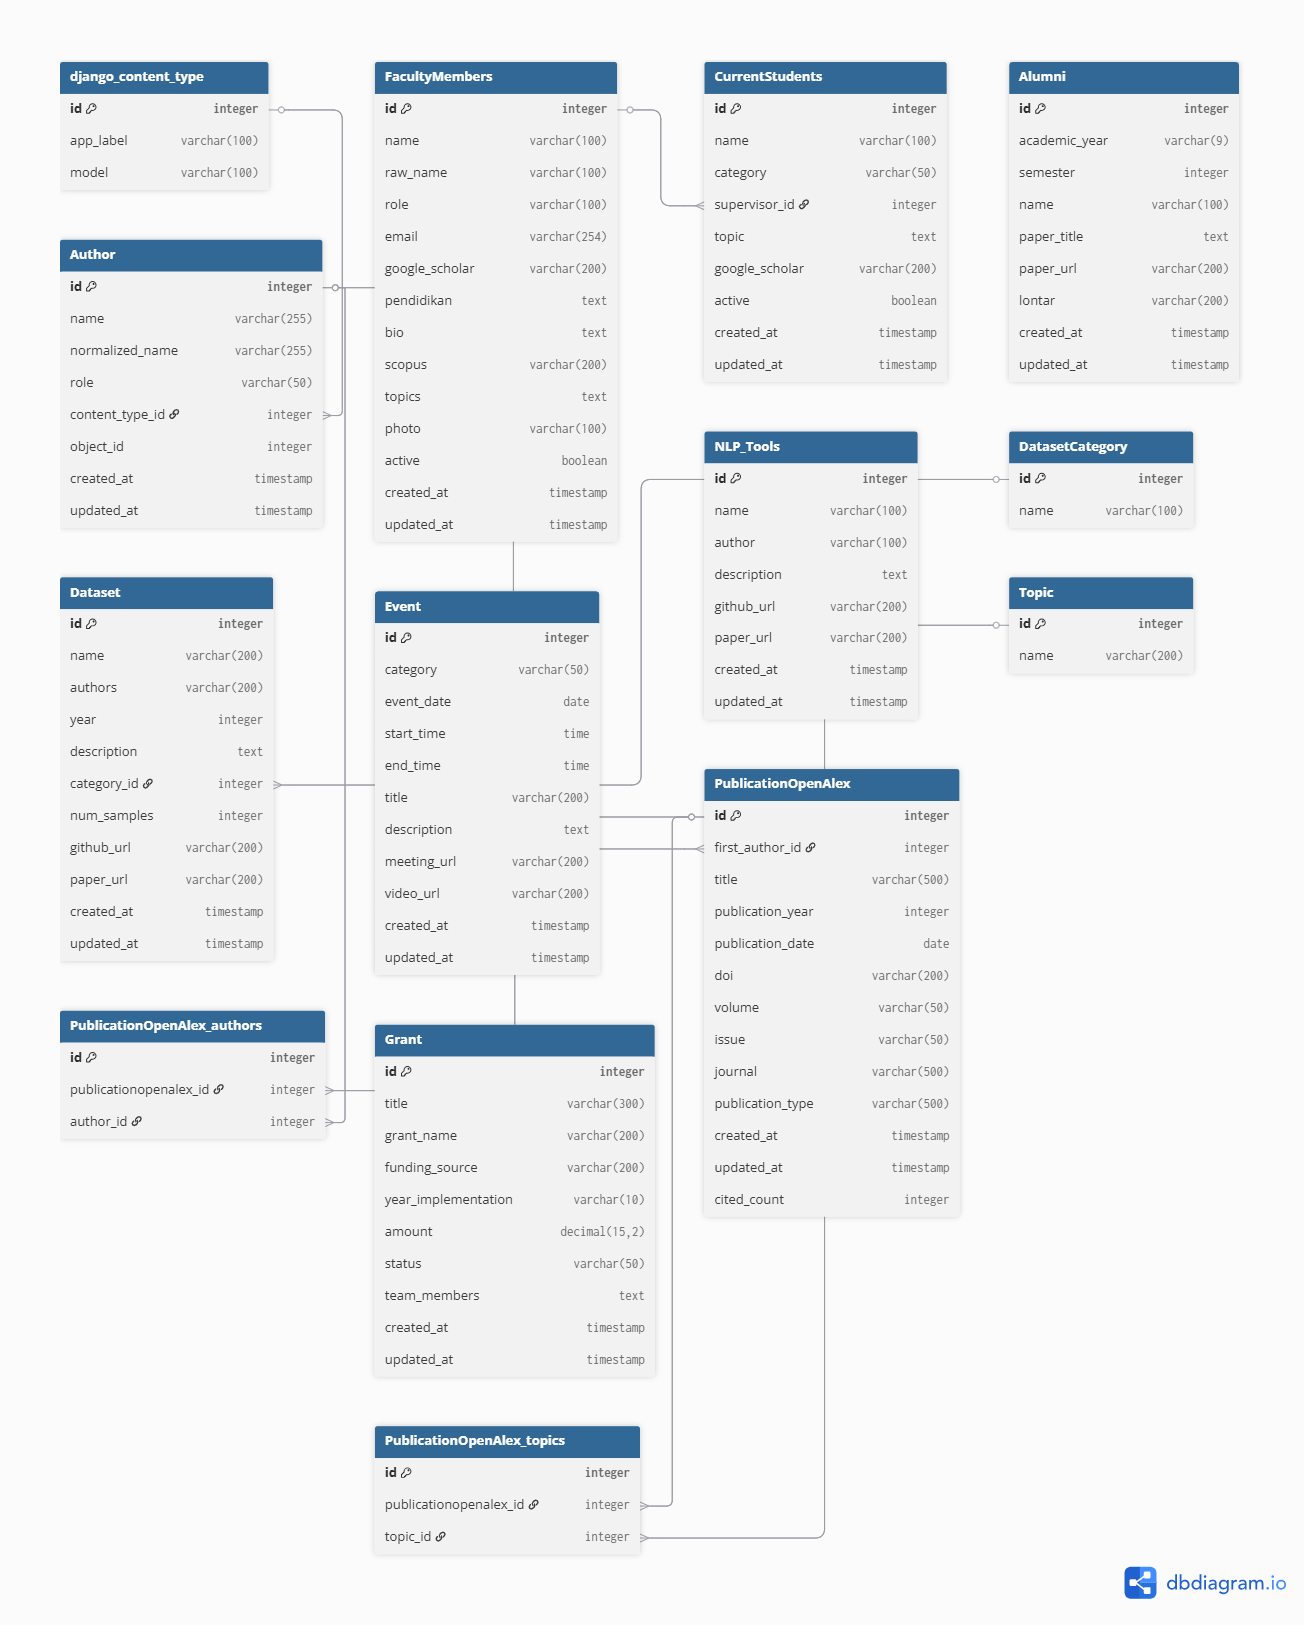
\includegraphics[width=\textwidth]{assets/pics/bab2_model_erd.png}
    \caption{Entity Relationship Diagram (ERD)}
    \label{fig:erd}
\end{figure}

\subsection{Deskripsi Model Anggota Lab}

Sistem ini dirancang untuk mengelola tiga kategori utama individu yang terkait dengan lingkungan akademik: 
\textit{Dosen} (\texttt{FacultyMembers}), \textit{Mahasiswa Aktif} (\texttt{CurrentStudents}), dan 
\textit{Alumni} (\texttt{Alumni}). Untuk menyatukan representasi individu-individu ini ketika mereka 
berperan sebagai penulis dalam publikasi, digunakan sebuah model pusat yang disebut \texttt{Author}.

Desain ini memungkinkan setiap individu memiliki profil detail sesuai perannya (misalnya, dosen memiliki 
riwayat pendidikan, mahasiswa memiliki pembimbing), sekaligus dapat diidentifikasi secara seragam sebagai 
seorang penulis tanpa duplikasi data.

\subsection{Deskripsi Entitas (Tabel)}

\subsubsection{FacultyMembers}
\textbf{Tujuan}: Menyimpan data profil lengkap dari para staf pengajar (dosen).

\textbf{Atribut Kunci}:
\begin{itemize}
    \item \textbf{id}: Pengenal unik untuk setiap dosen.
    \item \textbf{name}: Nama lengkap dosen.
    \item \textbf{role}: Status kepegawaian (misalnya, ``Staf Pengajar Tetap'').
    \item \textbf{email}: Alamat email kontak.
\end{itemize}

\subsubsection{CurrentStudents}
\textbf{Tujuan}: Mengelola data mahasiswa yang sedang menempuh studi.

\textbf{Atribut Kunci}:
\begin{itemize}
    \item \textbf{id}: Pengenal unik untuk setiap mahasiswa.
    \item \textbf{name}: Nama lengkap mahasiswa.
    \item \textbf{category}: Jenjang studi (misalnya, ``Doctoral Student'').
    \item \textbf{supervisor\_id}: \textit{Foreign Key} yang merujuk ke \texttt{FacultyMembers.id}, 
    menandakan dosen pembimbing.
\end{itemize}

\subsubsection{Alumni}
\textbf{Tujuan}: Menyimpan arsip data mahasiswa yang telah lulus.

\textbf{Atribut Kunci}:
\begin{itemize}
    \item \textbf{id}: Pengenal unik untuk setiap alumni.
    \item \textbf{name}: Nama lengkap alumni.
    \item \textbf{academic\_year}: Tahun ajaran kelulusan.
\end{itemize}

\subsubsection{Author}
\textbf{Tujuan}: Bertindak sebagai jembatan atau representasi generik dari seorang penulis. 
Entitas ini tidak menyimpan detail pribadi, melainkan hanya nama dan mekanisme untuk terhubung 
ke profil aslinya.

\textbf{Atribut Kunci}:
\begin{itemize}
    \item \textbf{id}: Pengenal unik untuk setiap entri penulis.
    \item \textbf{name}: Nama penulis seperti yang tertera di publikasi.
    \item \textbf{role}: Peran penulis (dosen, mahasiswa, dll.).
    \item \textbf{content\_type\_id} dan \textbf{object\_id}: Kolom untuk relasi 
    polimorfik menggunakan mekanisme \textit{Generic Foreign Key}.
\end{itemize}

\subsubsection{django\_content\_type}
\textbf{Tujuan}: Tabel bawaan Django yang berfungsi sebagai kamus model. Tabel ini menyimpan daftar 
semua model (tabel) yang ada di dalam sistem, sehingga \texttt{Author} dapat mengetahui profil mana 
yang harus dirujuk.

\subsection{Deskripsi Publikasi}
Sistem manajemen publikasi dilakukan dengan scraping dan dapat dilakukan pengeditan pada publikasi tersebut ketika terjadi kesalahan.

\begin{itemize}
   
    \item \textbf{Alur Otomatis (PublicationOpenAlex)}: 
    Untuk pengumpulan data massal dari sumber eksternal (OpenAlex) secara otomatis, dengan metadata yang 
    lebih kaya dan sistem klasifikasi berbasis topik.
\end{itemize}

Kedua alur ini terintegrasi melalui entitas \texttt{Author}, yang memastikan bahwa setiap publikasi dari 
sumber manapun dapat ditautkan kembali ke profil individu yang relevan.

% ---------------------------------------------------------------------------

\subsection{Deskripsi Entitas (Tabel)}

\subsubsection*{Entitas Pusat}
\begin{itemize}
    \item \textbf{Author}: Berperan sebagai penghubung utama. 
    Setiap entri di \texttt{Publications} dan \texttt{PublicationOpenAlex} harus terhubung 
    ke satu atau lebih \texttt{Author}.
\end{itemize}

\subsubsection*{Entitas dalam Publikasi}
\begin{itemize}
    \item \textbf{PublicationOpenAlex}: 
    Tabel untuk menyimpan hasil scraping. Memiliki atribut kaya seperti \texttt{doi}, 
    \texttt{cited\_count}, \texttt{publication\_year}, dan \texttt{journal}.
    
    \item \textbf{Topic}: 
    Menyimpan daftar topik penelitian (misalnya, ``Machine Learning'', ``Sentiment Analysis'') 
    yang digunakan untuk mengklasifikasikan publikasi dari OpenAlex.
\end{itemize}

\subsubsection*{Entitas Perantara (Junction Tables)}
\begin{itemize}
    \item \textbf{publications\_authors}: Menghubungkan \texttt{Publications} dan \texttt{Author} 
    dalam relasi many-to-many.
    
    \item \textbf{publicationopenalex\_authors}: Menghubungkan \texttt{PublicationOpenAlex} 
    dan \texttt{Author} dalam relasi many-to-many.
    
    \item \textbf{publicationopenalex\_topics}: Menghubungkan \texttt{PublicationOpenAlex} 
    dan \texttt{Topic} dalam relasi many-to-many.
\end{itemize}

% ---------------------------------------------------------------------------

\subsection{Deskripsi Relasi}

\subsubsection*{Relasi Penulisan (Many-to-Many)}
Baik \texttt{Publications} maupun \texttt{PublicationOpenAlex} memiliki relasi many-to-many dengan \texttt{Author}.  
\textit{Arti}: Satu publikasi dapat ditulis oleh banyak penulis, dan satu penulis dapat menulis banyak publikasi.  
Relasi ini diimplementasikan melalui tabel perantara \texttt{publications\_authors} dan 
\texttt{publicationopenalex\_authors}. Ini adalah relasi paling fundamental dalam diagram ini.

\subsubsection*{Relasi Klasifikasi Hirarkis (Alur Manual)}
Hubungan antara \texttt{MajorCategoryPublications} $\rightarrow$ 
\texttt{SubCategoryPublications} $\rightarrow$ \texttt{Publications} bersifat hirarkis dan bertingkat.

\begin{itemize}
    \item \textbf{MajorCategoryPublications ke SubCategoryPublications (One-to-Many)}:  
    Satu kategori utama dapat memiliki banyak sub-kategori.
    
    \item \textbf{SubCategoryPublications ke Publications (One-to-Many)}:  
    Satu sub-kategori dapat diterapkan pada banyak publikasi manual.  
    Hal ini menciptakan struktur klasifikasi yang rapi dan terkontrol.
\end{itemize}

\subsubsection*{Relasi Klasifikasi Berbasis Tag (Alur Otomatis)}
\textbf{PublicationOpenAlex ke Topic (Many-to-Many)}:

\textit{Arti}: Satu publikasi otomatis bisa memiliki banyak topik (mirip sistem tag), dan satu topik dapat 
terhubung ke banyak publikasi. Relasi ini lebih fleksibel dan cocok untuk metadata kaya dari OpenAlex.

\subsubsection*{Relasi Khusus Penulis Pertama (One-to-Many)}
\textbf{PublicationOpenAlex ke Author (melalui \texttt{first\_author\_id})}:

\textit{Arti}:  
Satu \texttt{Author} bisa menjadi penulis pertama untuk banyak publikasi,  
tetapi setiap entri \texttt{PublicationOpenAlex} hanya memiliki satu \texttt{first\_author}.  
Relasi ini merupakan optimisasi untuk memudahkan identifikasi kontributor utama.

\subsection{Deskripsi Model Acara}
Modul Manajemen Acara dirancang sebagai sistem yang mandiri (\textit{self-contained}) 
untuk mengelola, mengumumkan, dan mengarsipkan seluruh kegiatan akademik seperti seminar, 
lokakarya, dan \textit{talk series}. Tujuan utamanya adalah menyediakan satu sumber 
informasi terpusat untuk semua acara yang diselenggarakan, mulai dari jadwal hingga 
materi pasca-acara.

Entitas tunggal dalam konteks ini adalah \texttt{Event}, yang menyimpan seluruh detail 
yang diperlukan untuk menginformasikan audiens tentang sebuah acara dari awal hingga akhir.

% --------------------------------------------------------------------

\subsection{Deskripsi Entitas (Tabel)}

\subsubsection{Event}

\textbf{Tujuan}: Menjadi catatan tunggal dan komprehensif untuk setiap acara. 
Setiap entri \texttt{Event} merepresentasikan satu acara unik.

\textbf{Atribut Kunci}:
\begin{itemize}
    \item \textbf{id}: Pengenal unik (Primary Key) untuk setiap acara.
    \item \textbf{title}: Judul atau nama resmi acara.
    \item \textbf{description}: Deskripsi lengkap mengenai acara, termasuk topik, nama pembicara, 
    dan detail relevan lainnya.
    \item \textbf{category}: Klasifikasi jenis acara (misalnya, ``IR-NLP Talks'', ``Seminar'') 
    untuk mempermudah penyaringan dan pengelompokan.
    \item \textbf{event\_date}, \textbf{start\_time}, \textbf{end\_time}: 
    Atribut temporal yang mencakup tanggal acara, waktu mulai, dan waktu selesai (opsional).
    \item \textbf{meeting\_url}: Tautan untuk mengikuti acara secara daring (Zoom, Google Meet), bersifat opsional.
    \item \textbf{video\_url}: Tautan rekaman video pasca-acara. Bersifat opsional.
\end{itemize}

% --------------------------------------------------------------------

\subsection{Deskripsi Relasi}

\subsubsection{Entitas Mandiri (Standalone Entity)}

Dalam skema yang didefinisikan, \texttt{Event} merupakan entitas yang berdiri sendiri. 
Tabel \texttt{Event} tidak memiliki hubungan \textit{foreign key} ke tabel lain seperti 
\texttt{FacultyMembers} (untuk pembicara) atau \texttt{Topic}.

\textbf{Implikasi Desain}:
Pendekatan ini menyederhanakan pengelolaan acara. Informasi pembicara, baik internal maupun 
eksternal, dapat langsung dicantumkan dalam kolom \texttt{description} tanpa perlu direlasikan 
secara formal ke entitas lain. Fleksibilitas ini sangat berguna ketika pembicara berasal dari 
luar institusi dan tidak tercatat dalam sistem.

\section{Perancangan Antarmuka}

Perancangan antarmuka dilakukan dengan terlebih dahulu mencari referensi desain halaman depan (landing page) melalui situs Pinterest. Dari proses pencarian tersebut, diperoleh beberapa referensi desain yang dijadikan acuan awal.

\begin{figure}[H]
    \centering
    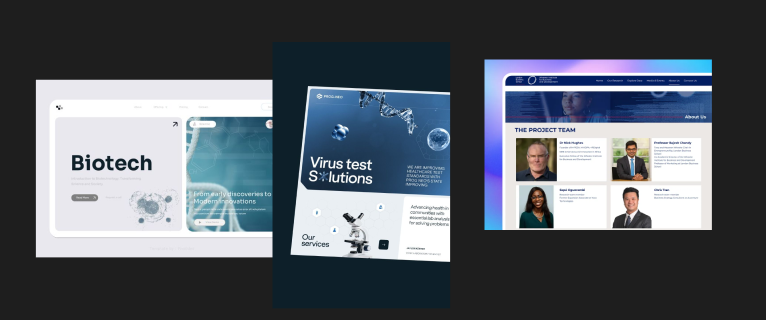
\includegraphics[width=0.7\textwidth]{assets/pics/bab2_referensi.png} % ganti dengan path gambar Anda
    \caption{Gambar Referensi Desain}
\end{figure}

Selanjutnya, proses perancangan dilakukan dengan membuat wireframe sebagai representasi awal tampilan antarmuka. Penggunaan wireframe dipilih karena bersifat fleksibel dan mudah disesuaikan berdasarkan masukan atau revisi yang muncul selama proses pengembangan.

Wireframe yang dirancang berfokus pada halaman utama (landing page), kemudian dibuat secara detail menggunakan Figma.

\begin{figure}[H]
    \centering
    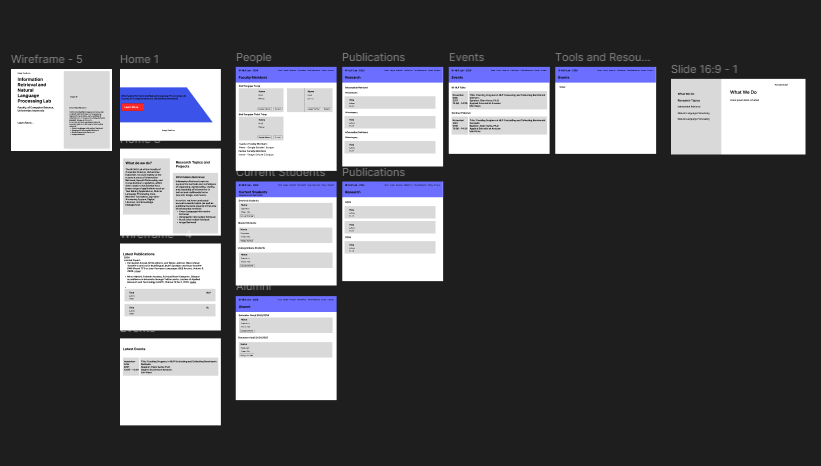
\includegraphics[width=0.7\textwidth]{assets/pics/bab2_wireframe.png} % ganti dengan path gambar Anda
    \caption{Wireframe Halaman Landing Page}
\end{figure}


%-----------------------------------------------------------------------------%
